\documentclass{report}
\usepackage{tikz}
\usepackage{subcaption}

\begin{document}
\begin{figure}
  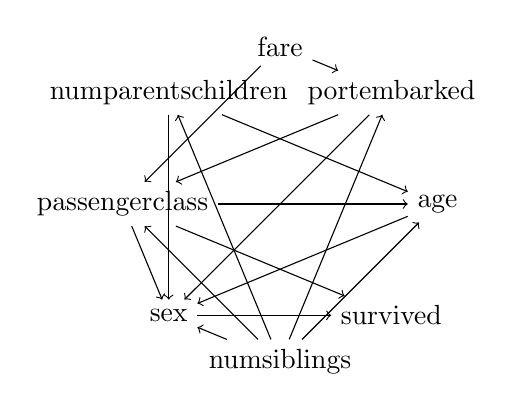
\begin{tikzpicture}
      \draw
        (0.0:2) node (age){age}
        (45.0:2) node (portembarked){portembarked}
        (90.0:2) node (fare){fare}
        (135.0:2) node (numparentschildren){numparentschildren}
        (180.0:2) node (passengerclass){passengerclass}
        (225.0:2) node (sex){sex}
        (270.0:2) node (numsiblings){numsiblings}
        (315.0:2) node (survived){survived};
      \begin{scope}[->]
        \draw (age) to (sex);
        \draw (portembarked) to (passengerclass);
        \draw (portembarked) to (sex);
        \draw (fare) to (portembarked);
        \draw (fare) to (passengerclass);
        \draw (numparentschildren) to (age);
        \draw (numparentschildren) to (sex);
        \draw (passengerclass) to (age);
        \draw (passengerclass) to (sex);
        \draw (passengerclass) to (survived);
        \draw (sex) to (survived);
        \draw (numsiblings) to (age);
        \draw (numsiblings) to (portembarked);
        \draw (numsiblings) to (numparentschildren);
        \draw (numsiblings) to (passengerclass);
        \draw (numsiblings) to (sex);
      \end{scope}
    \end{tikzpicture}
  \caption{small}
\end{figure}
\end{document}